%%%%%%
%
% Ergebnispräsentation ELMAR Heiß Drahtschneider
%
%%%%%%

\Mysection{Projektmanagement}

\STANDARD{Vorgaben der Ergebnispräsentation}
{
  \begin{columns}[T]
    \begin{column}{0.48\textwidth}
      \begin{block}{Inhaltliche Schwerpunkte}
        \begin{itemize}
          \item LaTeX-Projekt als durchgängige Dokumentationsgrundlage
          \item eigene Bilder mit TikZ für technische Zusammenhänge
          \item Problembeschreibung und Beschreibung der Anwendung
          \item Herausforderungen, eigene Lösungen und Ergebnisse
        \end{itemize}
      \end{block}
    \end{column}
    \begin{column}{0.48\textwidth}
      \begin{block}{Ziel der Präsentation}
        Die Präsentation fasst den erreichten Projektstand des ELMAR Heiß Drahtschneiders zusammen und zeigt, wie Konstruktion, Elektronik, Software und Dokumentation zu einem funktionierenden Gesamtsystem verbunden wurden.
      \end{block}
    \end{column}
  \end{columns}
}

\STANDARD{LaTeX-Projekt und eigene Darstellungen}
{
  \begin{columns}[T]
    \begin{column}{0.52\textwidth}
      \begin{block}{LaTeX-Projekt}
        \begin{itemize}
          \item technische Dokumentation, Handbuch, Montageanleitung und Präsentation wurden als LaTeX-basierte Unterlagen aufgebaut
          \item Kapitel, Bilder, Tabellen, Quellcode und Literaturquellen sind dadurch einheitlich strukturiert
          \item Änderungen können gezielt in einzelnen Dateien gepflegt werden
        \end{itemize}
      \end{block}
    \end{column}
    \begin{column}{0.42\textwidth}
      \begin{block}{Eigene Bilder mit TikZ}
        \begin{itemize}
          \item Systemübersichten und Ablaufdarstellungen wurden als eigene TikZ-Grafiken erstellt
          \item dadurch passen die Grafiken optisch zur Dokumentation
          \item technische Signalwege und Baugruppen werden verständlicher dargestellt
        \end{itemize}
      \end{block}
    \end{column}
  \end{columns}
}

\Mysection{Problem und Anwendung}

\STANDARD{Problembeschreibung}
{
  \begin{columns}[T]
    \begin{column}{0.55\textwidth}
      \begin{block}{Ausgangssituation}
        \begin{itemize}
          \item Styropor wird im Modellbau häufig verwendet, ist manuell aber schwer exakt zu schneiden.
          \item Handgeführte Heiß Drahtschneider erfordern eine ruhige Hand und führen nur bedingt zu wiederholbaren Konturen.
          \item Ziel war ein automatisierter Heiß Drahtschneider, der Konturen aus G-Code reproduzierbar abfährt.
        \end{itemize}
      \end{block}
    \end{column}
    \begin{column}{0.40\textwidth}
      \begin{figure}
        \centering
        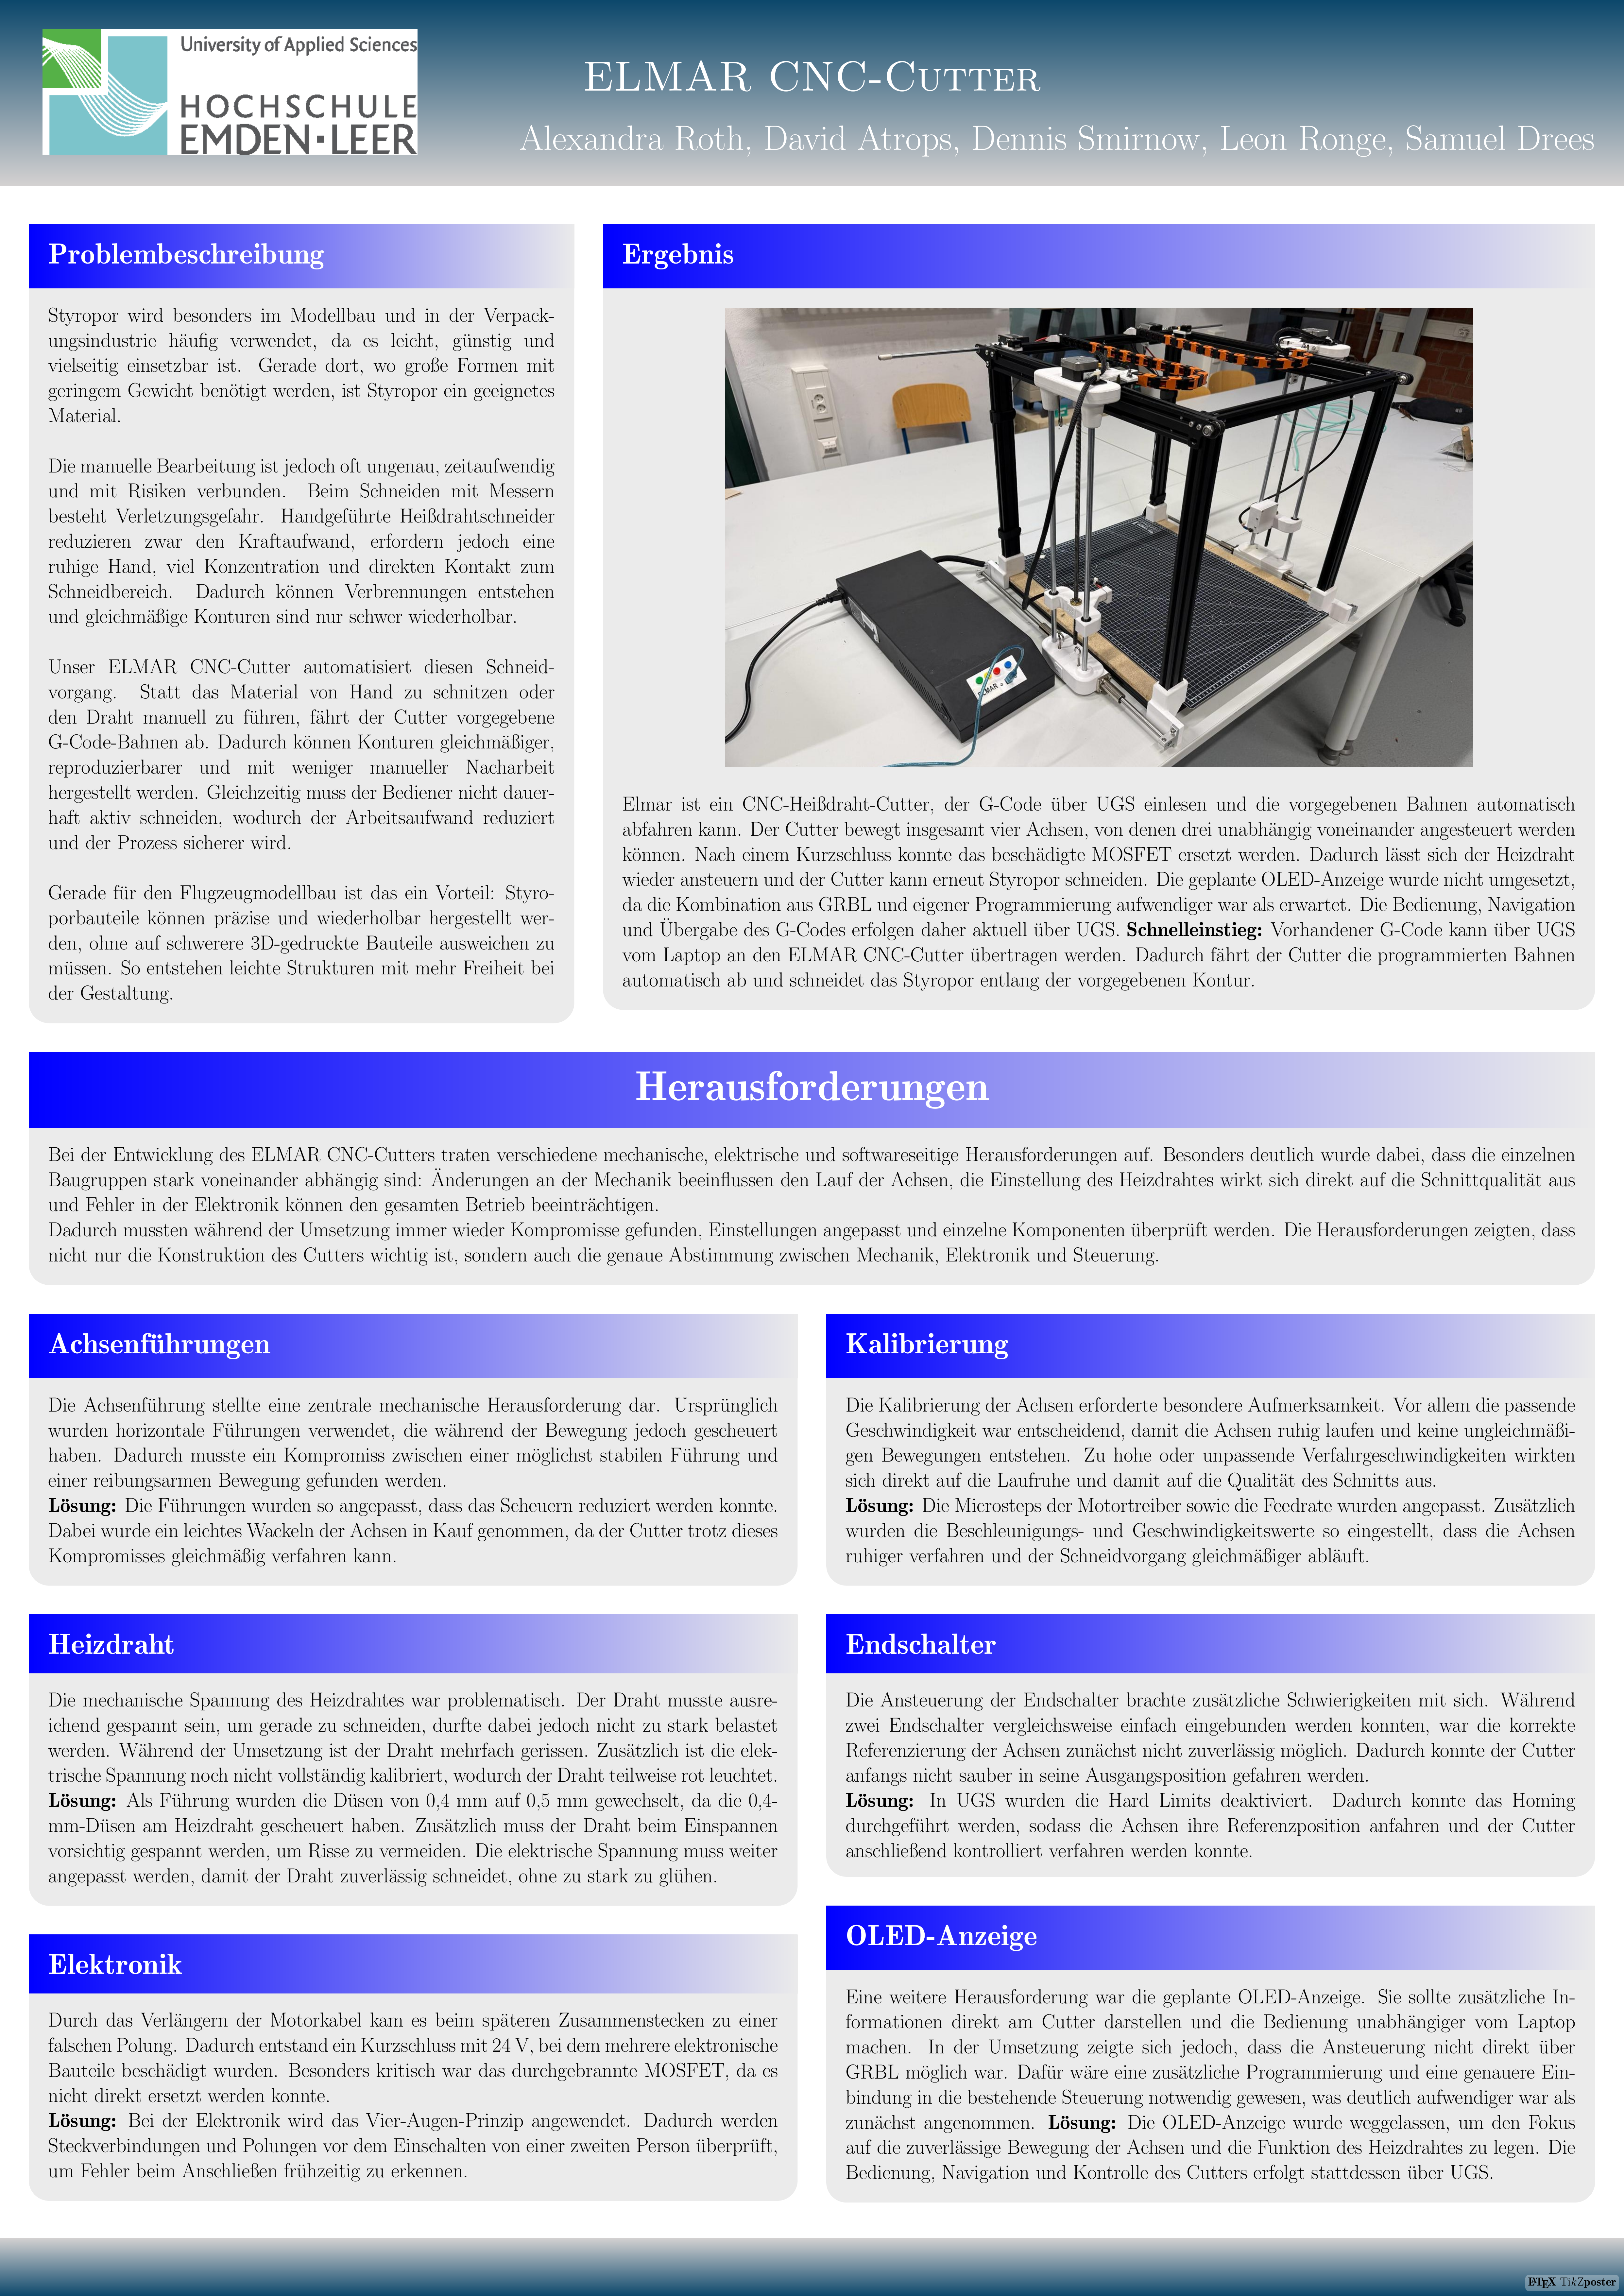
\includegraphics[width=0.96\textwidth]{images/poster}
      \end{figure}
    \end{column}
  \end{columns}
}

\STANDARD{Beschreibung der Anwendung}
{
  \begin{block}{Kernidee}
    Der ELMAR Heiß Drahtschneider bewegt einen Heizdraht automatisch entlang einer digitalen Schnittkontur und stellt dadurch leichte Styroporbauteile reproduzierbar her.
  \end{block}

  \vspace{0.3cm}
  \begin{columns}[T]
    \begin{column}{0.32\textwidth}
      \begin{block}{Mechanik}
        Rahmen, Führungen, Wagen und gespannter Heizdraht bilden den Schneidaufbau.
      \end{block}
    \end{column}
    \begin{column}{0.32\textwidth}
      \begin{block}{Elektronik}
        Arduino, CNC-Shield, Motortreiber, Endschalter und MOSFET steuern Achsen und Heizdraht.
      \end{block}
    \end{column}
    \begin{column}{0.32\textwidth}
      \begin{block}{Software}
        UGS überträgt G-Code an GRBL, welches die Schrittmotorbewegungen erzeugt.
      \end{block}
    \end{column}
  \end{columns}
}

\Mysection{Aufbau und Funktion}

\STANDARD{Systemaufbau}
{
  \begin{columns}[T]
    \begin{column}{0.58\textwidth}
      \begin{itemize}
        \item Vier Achsen bewegen den Heizdraht relativ zum Schaumstoffblock.
        \item Drei Achsen können unabhängig voneinander angesteuert werden.
        \item Endschalter unterstützen die Referenzfahrt und Positionsbestimmung.
        \item Das MOSFET-PWM-Schaltmodul übernimmt die Lastansteuerung des Heizdrahts.
      \end{itemize}
    \end{column}
    \begin{column}{0.38\textwidth}
      \begin{figure}
        \centering
        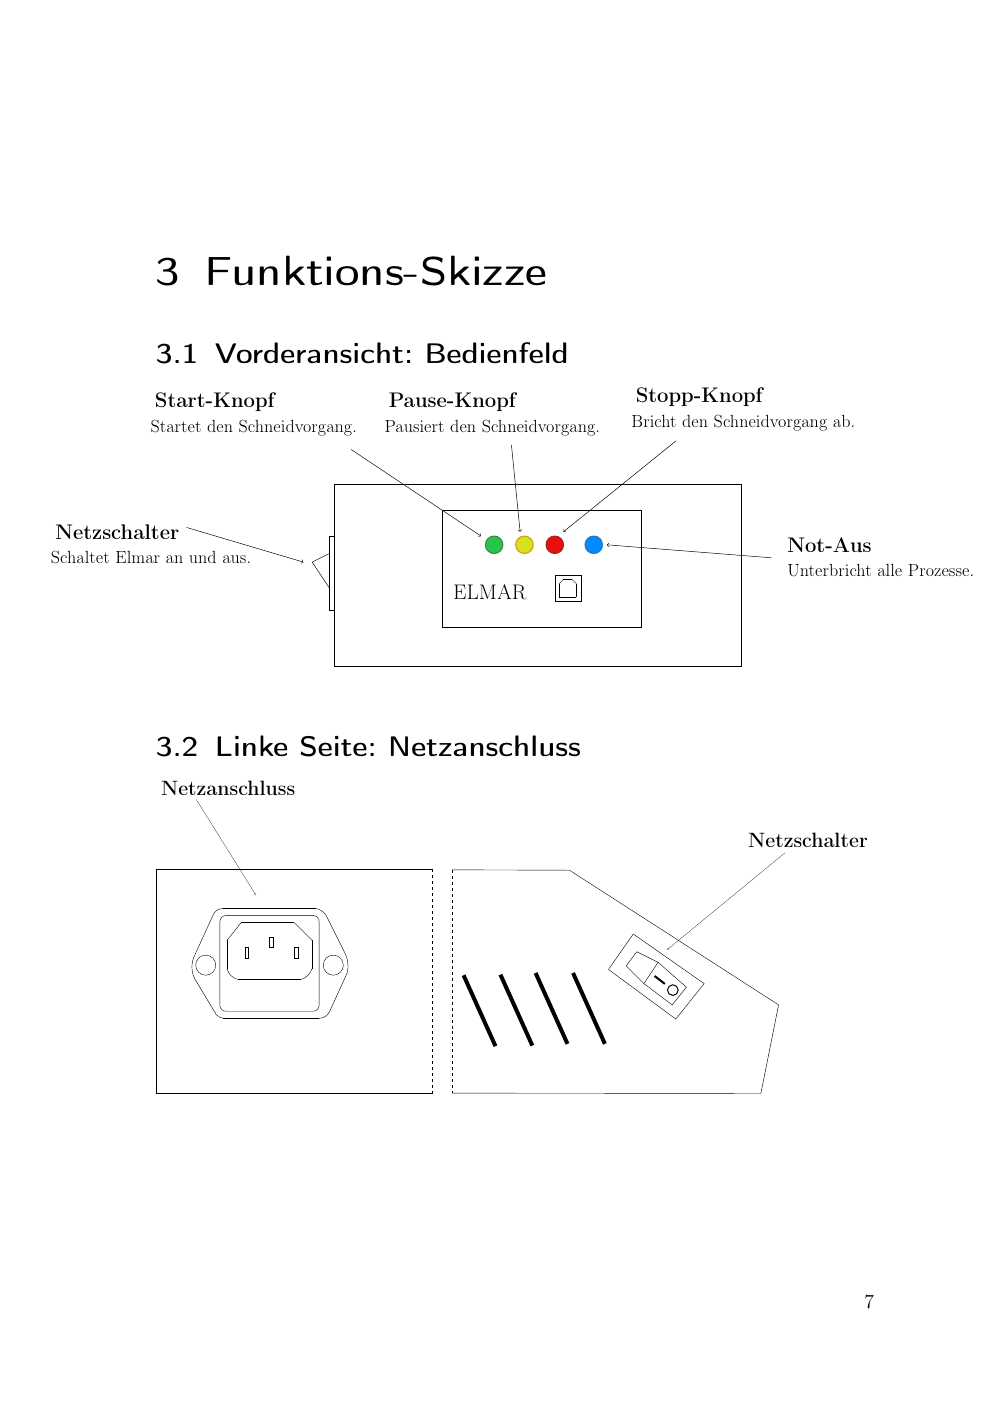
\includegraphics[width=0.95\textwidth]{images/handbuch_skizze}
      \end{figure}
    \end{column}
  \end{columns}
}

\STANDARD{Bedien- und Softwarekette}
{
  \begin{columns}[T]
    \begin{column}{0.50\textwidth}
      \begin{block}{Ablauf}
        \begin{enumerate}
          \item Kontur als G-Code vorbereiten
          \item Maschine verbinden und referenzieren
          \item Werkstück-Nullpunkt setzen
          \item Datei über UGS senden
          \item Heizdraht schneidet die Kontur ab
        \end{enumerate}
      \end{block}
    \end{column}
    \begin{column}{0.45\textwidth}
      \begin{block}{Verwendete Software}
        \begin{itemize}
          \item Arduino IDE für Upload und Tests
          \item GRBL als Firmware auf dem Arduino Uno
          \item Universal G-Code Sender als Bedienoberfläche
        \end{itemize}
      \end{block}
    \end{column}
  \end{columns}
}

\STANDARD{Inbetriebnahme}
{
  \begin{columns}[T]
    \begin{column}{0.53\textwidth}
      \begin{itemize}
        \item Stromversorgung, PC und UGS starten
        \item Serielle Verbindung zu GRBL herstellen
        \item Referenzfahrt / Homing ausführen
        \item Heizdrahttemperatur und Vorschub abstimmen
        \item Testfahrt und anschließend Schnitt durchführen
      \end{itemize}
    \end{column}
    \begin{column}{0.42\textwidth}
      \begin{figure}
        \centering
        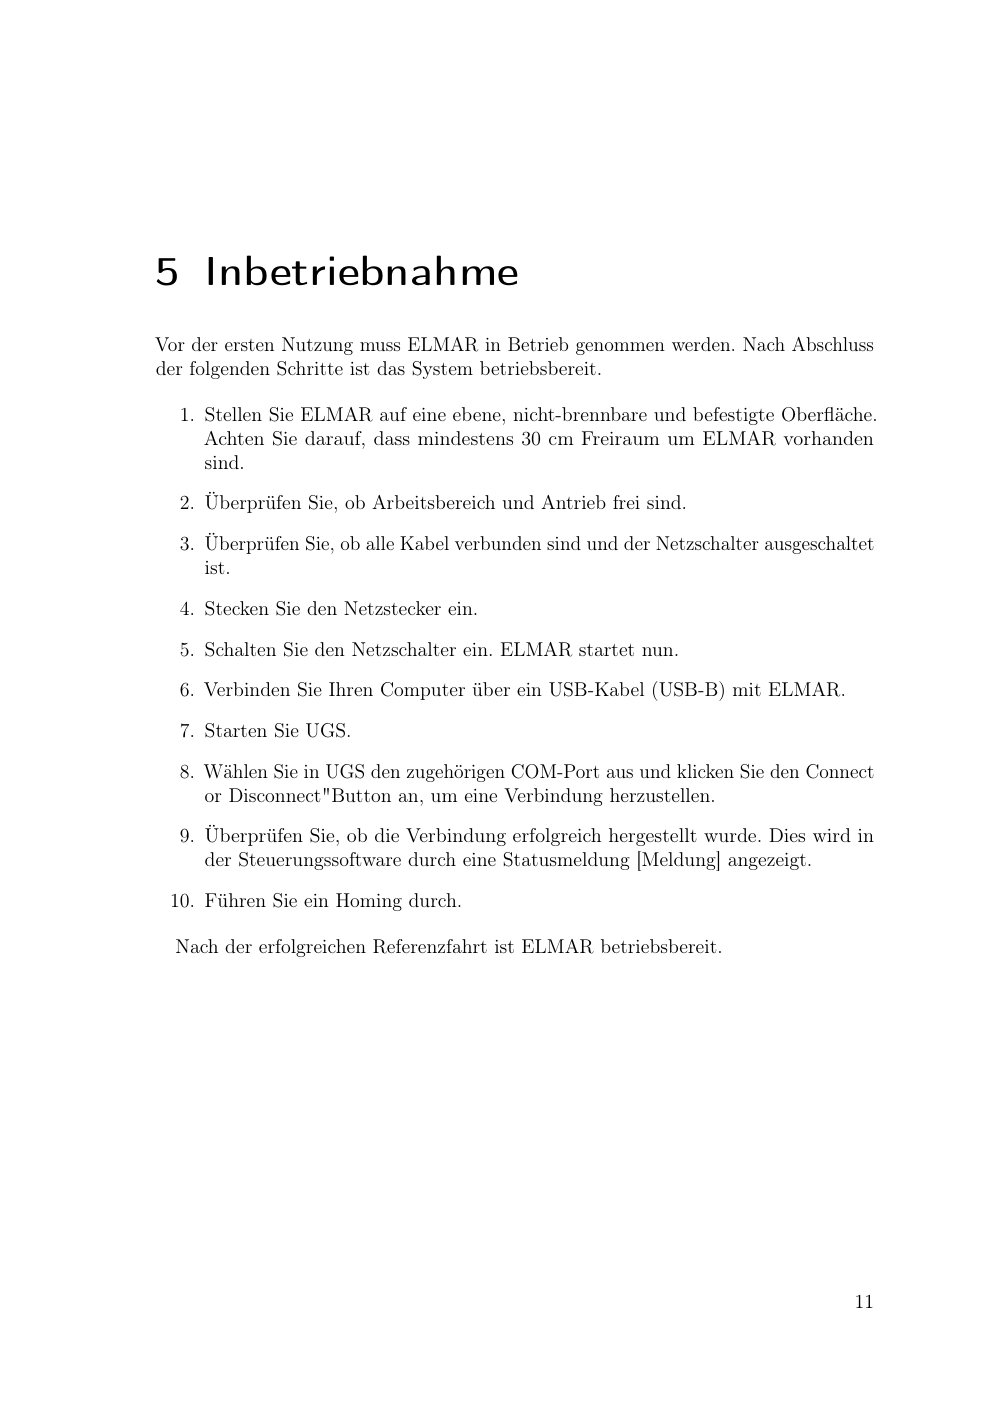
\includegraphics[width=0.92\textwidth]{images/inbetriebnahme}
      \end{figure}
    \end{column}
  \end{columns}
}

\Mysection{Montage}

\STANDARD{Mechanische Baugruppen}
{
  \begin{columns}[T]
    \begin{column}{0.48\textwidth}
      \begin{block}{Aufbau}
        \begin{itemize}
          \item Grundrahmen als stabile Basis
          \item Vertikalwagen links und rechts
          \item Horizontalwagen zur Führung des Schneiddrahts
          \item Riemen, Motoren, Endschalter und Drahtführung
        \end{itemize}
      \end{block}
    \end{column}
    \begin{column}{0.48\textwidth}
      \begin{figure}
        \centering
        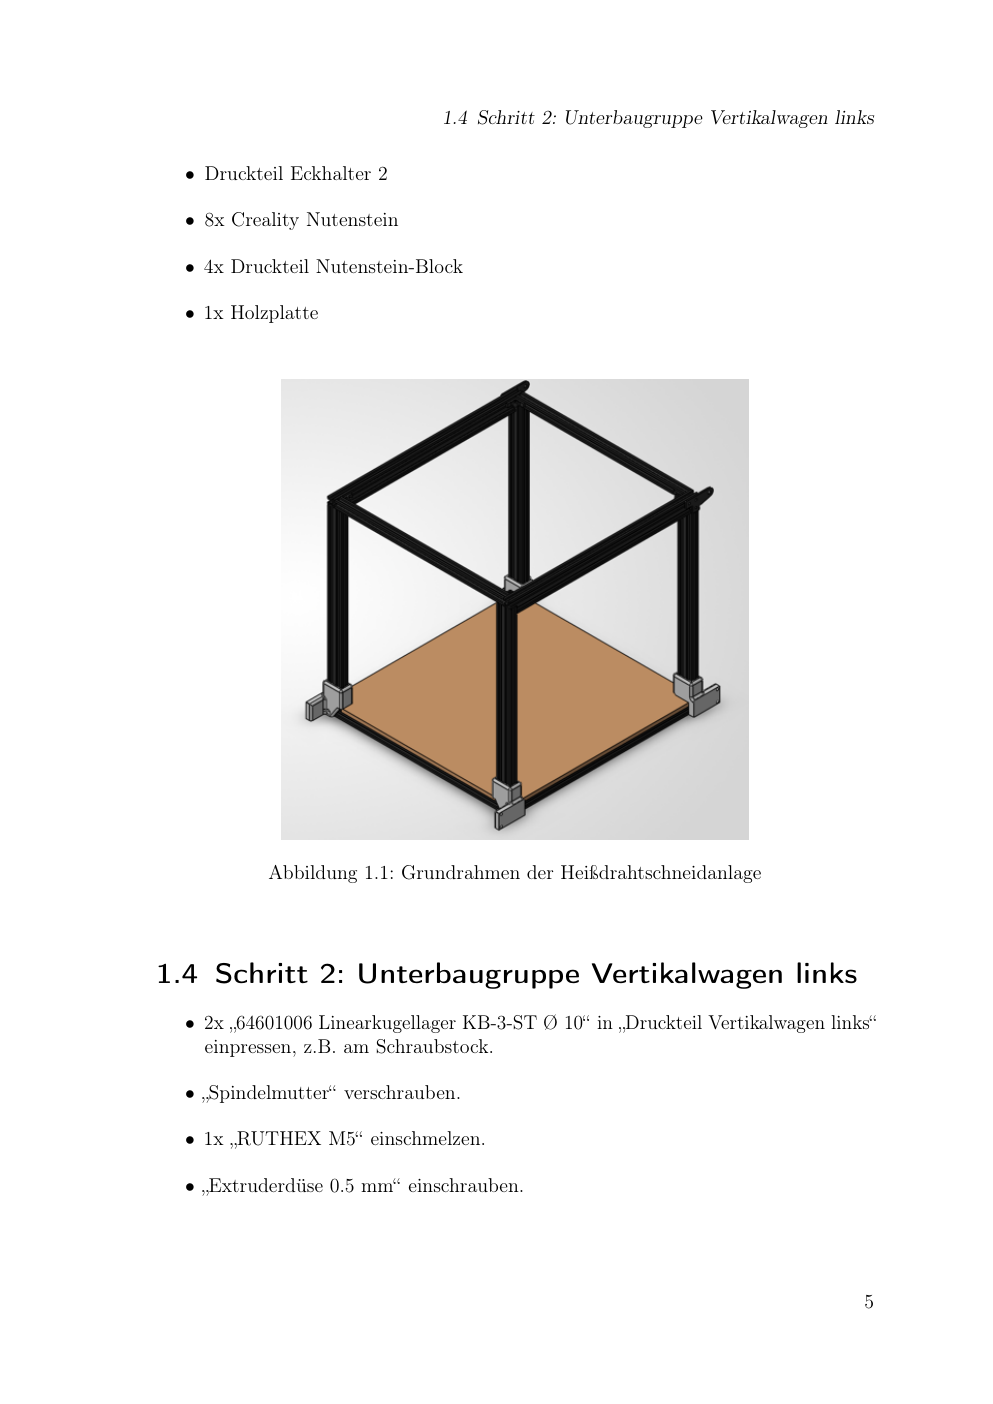
\includegraphics[width=0.95\textwidth]{images/montage_grundrahmen}
      \end{figure}
    \end{column}
  \end{columns}
}

\STANDARD{Montageeindrücke aus der Anleitung}
{
  \begin{columns}[T]
    \begin{column}{0.31\textwidth}
      \centering
      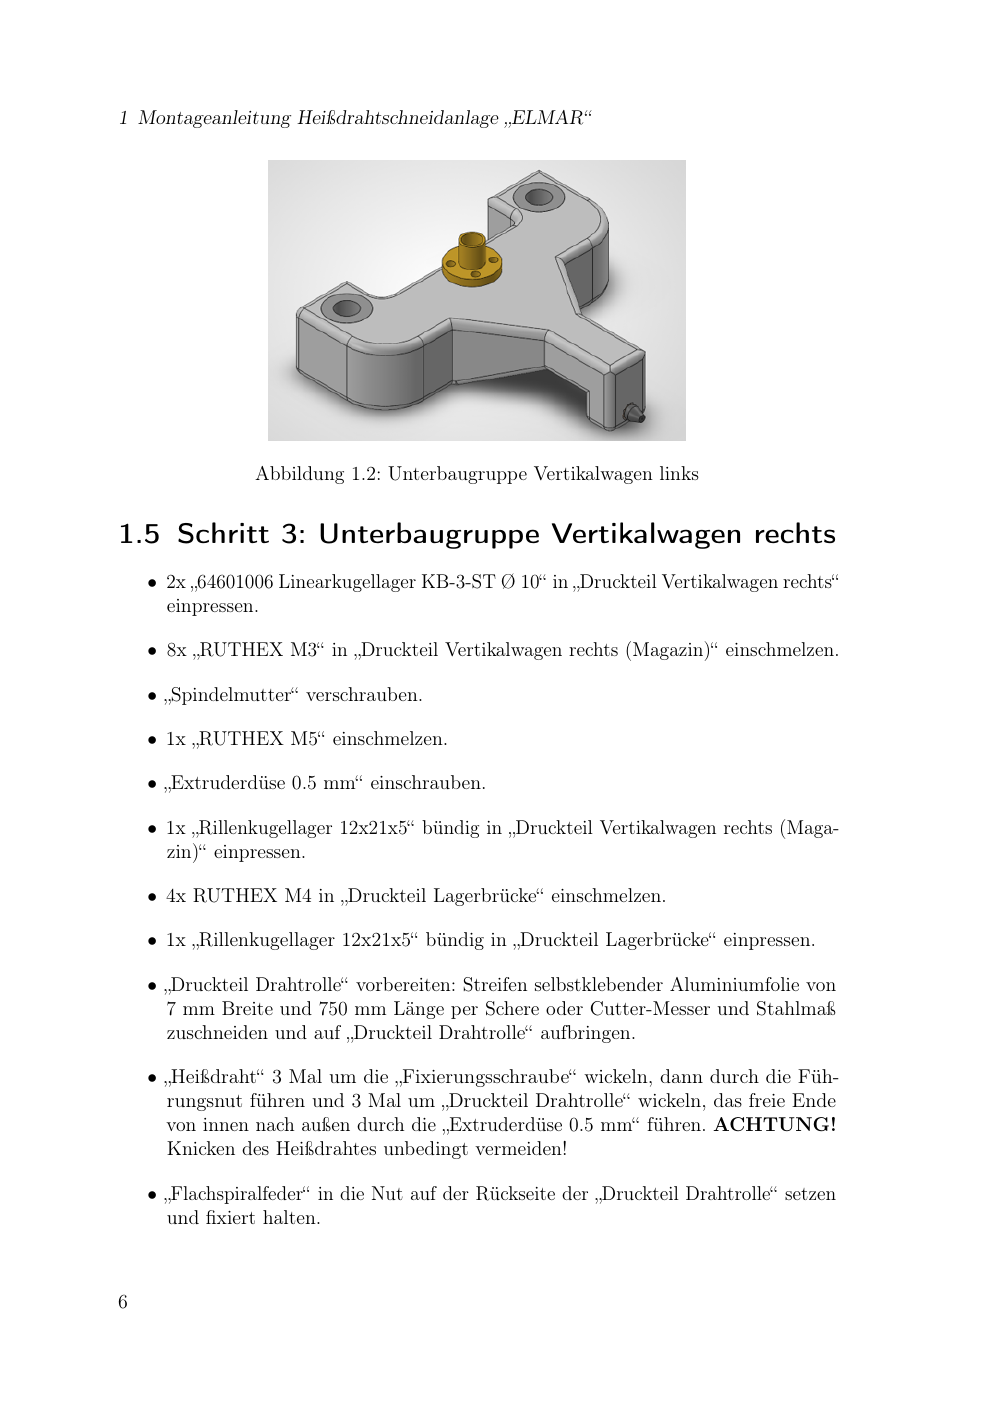
\includegraphics[width=0.95\textwidth]{images/montage_vertikal_links}
      \\ \scriptsize Vertikalwagen
    \end{column}
    \begin{column}{0.31\textwidth}
      \centering
      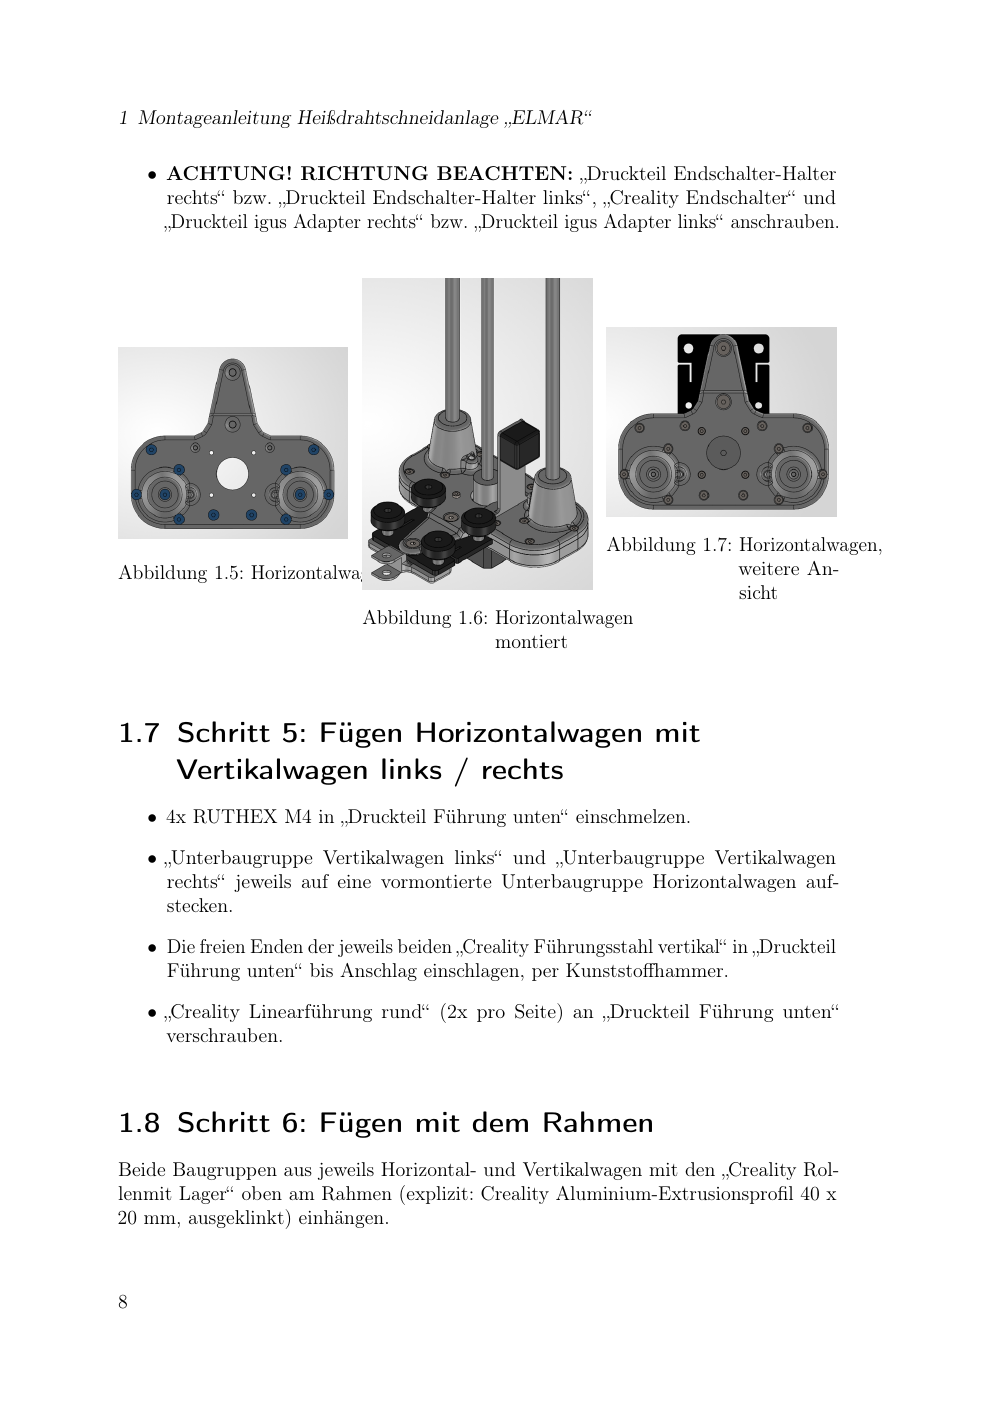
\includegraphics[width=0.95\textwidth]{images/montage_horizontal}
      \\ \scriptsize Horizontalwagen
    \end{column}
    \begin{column}{0.31\textwidth}
      \centering
      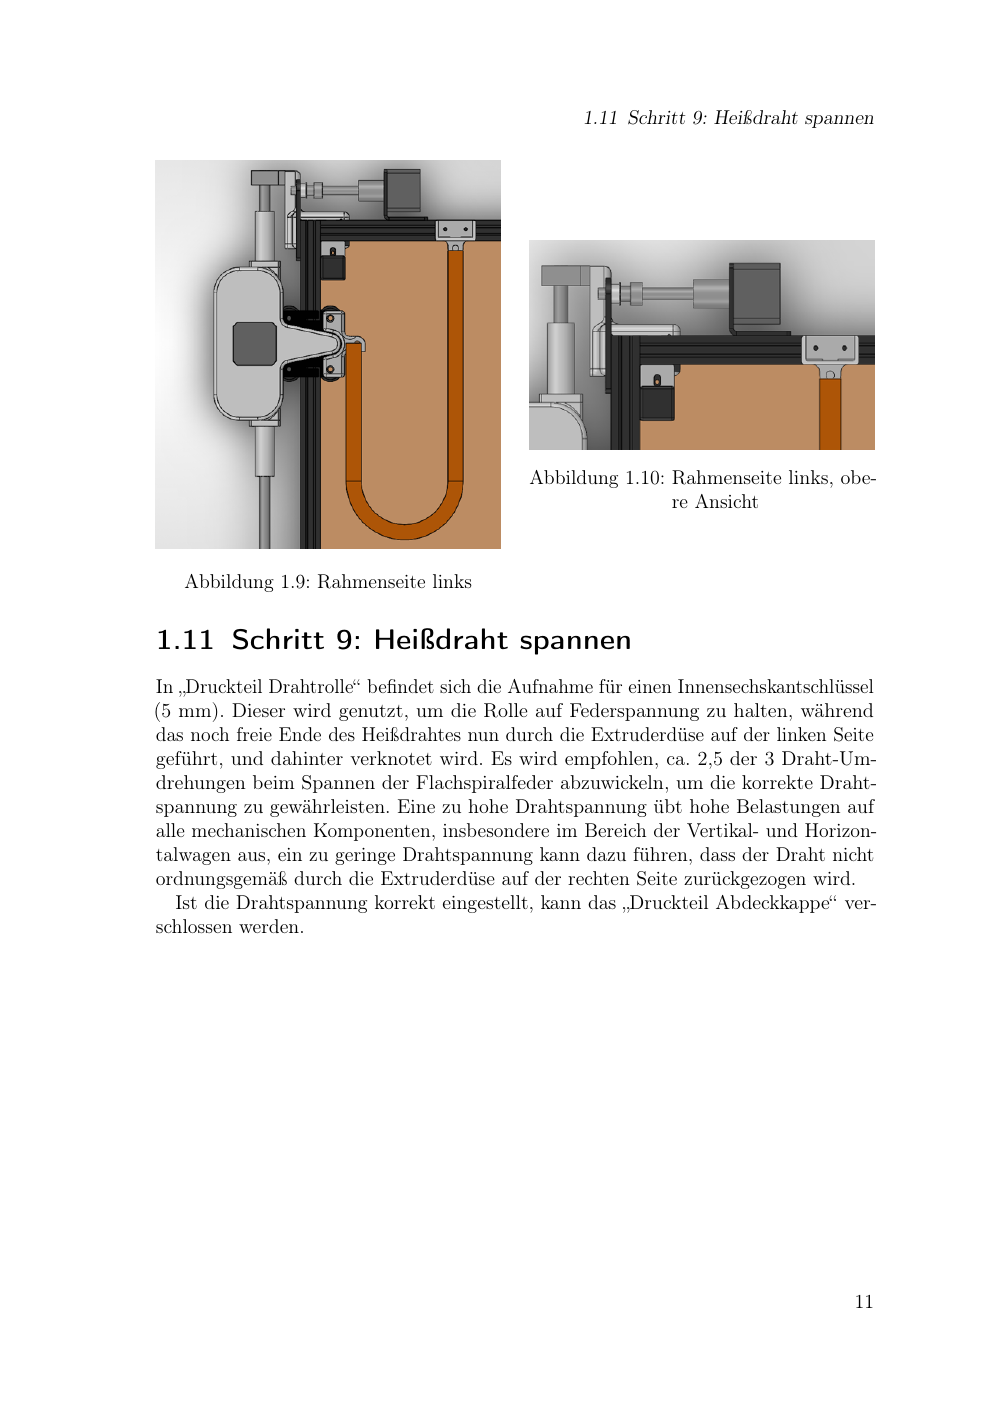
\includegraphics[width=0.95\textwidth]{images/montage_draht}
      \\ \scriptsize Drahtführung
    \end{column}
  \end{columns}
}

\Mysection{Herausforderungen und Lösungen}

\STANDARD{Zentrale Herausforderungen}
{
  \begin{columns}[T]
    \begin{column}{0.48\textwidth}
      \begin{block}{Mechanik}
        \begin{itemize}
          \item Achsführungen mussten zwischen Stabilität und Reibung abgestimmt werden.
          \item Der Heizdraht musste ausreichend gespannt werden, ohne zu reißen.
        \end{itemize}
      \end{block}
      \begin{block}{Kalibrierung}
        \begin{itemize}
          \item Microsteps, Feedrate, Beschleunigung und Geschwindigkeit wurden angepasst.
        \end{itemize}
      \end{block}
    \end{column}
    \begin{column}{0.48\textwidth}
      \begin{block}{Elektronik}
        \begin{itemize}
          \item Ein beschädigtes MOSFET musste ersetzt werden.
          \item Heizdrahtleistung und Vorschub mussten aufeinander abgestimmt werden.
        \end{itemize}
      \end{block}
      \begin{block}{Software}
        \begin{itemize}
          \item GRBL und eigene OLED-Programmierung ließen sich nicht wie geplant kombinieren.
          \item Bedienung erfolgt daher über UGS.
        \end{itemize}
      \end{block}
    \end{column}
  \end{columns}
}

\STANDARD{Eigene Lösungen}
{
  \begin{columns}[T]
    \begin{column}{0.48\textwidth}
      \begin{block}{Konstruktive Lösungen}
        \begin{itemize}
          \item eigene Halterungen und Wagen für den Schneidaufbau
          \item gespannte Drahtführung für eine gleichmäßige Schnittlinie
          \item modulare Baugruppen für Montage und Wartung
        \end{itemize}
      \end{block}
    \end{column}
    \begin{column}{0.48\textwidth}
      \begin{block}{Steuerung und Bedienung}
        \begin{itemize}
          \item GRBL als stabile Echtzeitsteuerung
          \item UGS für Verbindung, Referenzfahrt und G-Code-Übertragung
          \item PWM-Ansteuerung des Heizdrahts über MOSFET-Modul
        \end{itemize}
      \end{block}
    \end{column}
  \end{columns}
}

\Mysection{Ergebnisse}

\STANDARD{Ergebnisstand}
{
  \begin{block}{Erreicht}
    \begin{itemize}
      \item Der Heiß Drahtschneider kann G-Code über UGS einlesen und automatisiert Bahnen abfahren.
      \item Nach dem Austausch des MOSFET lässt sich der Heizdraht wieder ansteuern.
      \item Styropor kann entlang der vorgegebenen Kontur geschnitten werden.
    \end{itemize}
  \end{block}

  \vspace{0.25cm}
  \begin{block}{Offene Punkte}
    \begin{itemize}
      \item Feinkalibrierung von Drahttemperatur und Vorschubgeschwindigkeit
      \item weitere Optimierung der Achsführung und Schnittqualität
      \item OLED-Anzeige wurde nicht umgesetzt und bleibt als mögliche Erweiterung offen
    \end{itemize}
  \end{block}
}

\Mysection{Fotoeindrücke}

\STANDARD{Fotoeindrücke - Aufbau}
{
  \begin{columns}[T]
    \begin{column}{0.32\textwidth}
      \centering
      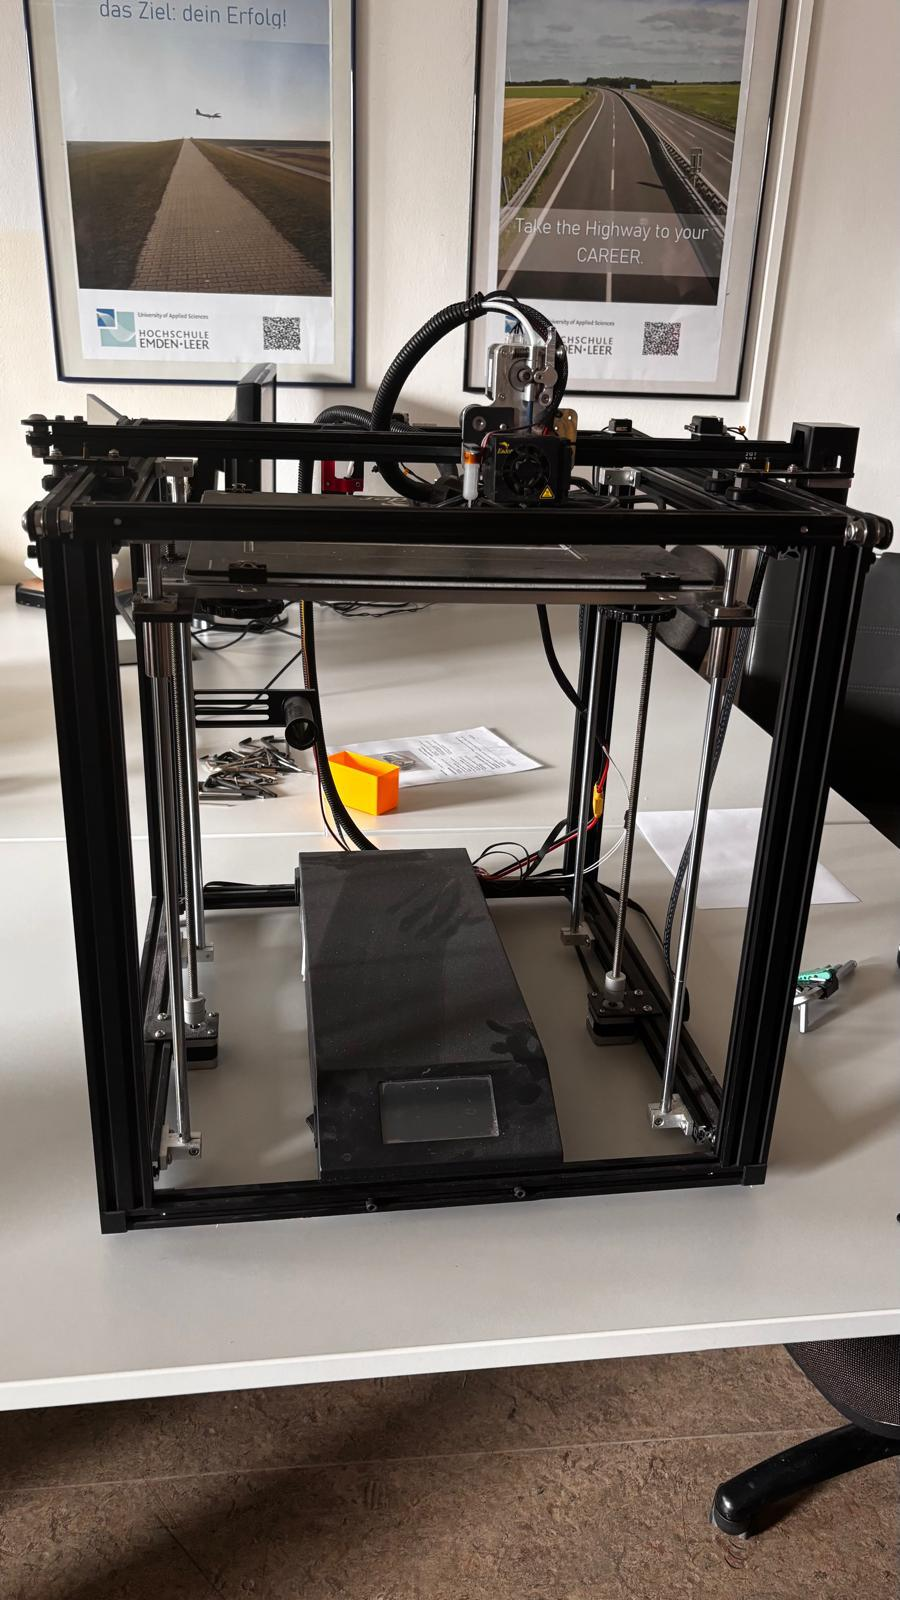
\includegraphics[height=4.7cm,width=\textwidth,keepaspectratio]{images/foto_gesamt_alt}
      \\ \scriptsize früher Aufbau
    \end{column}
    \begin{column}{0.32\textwidth}
      \centering
      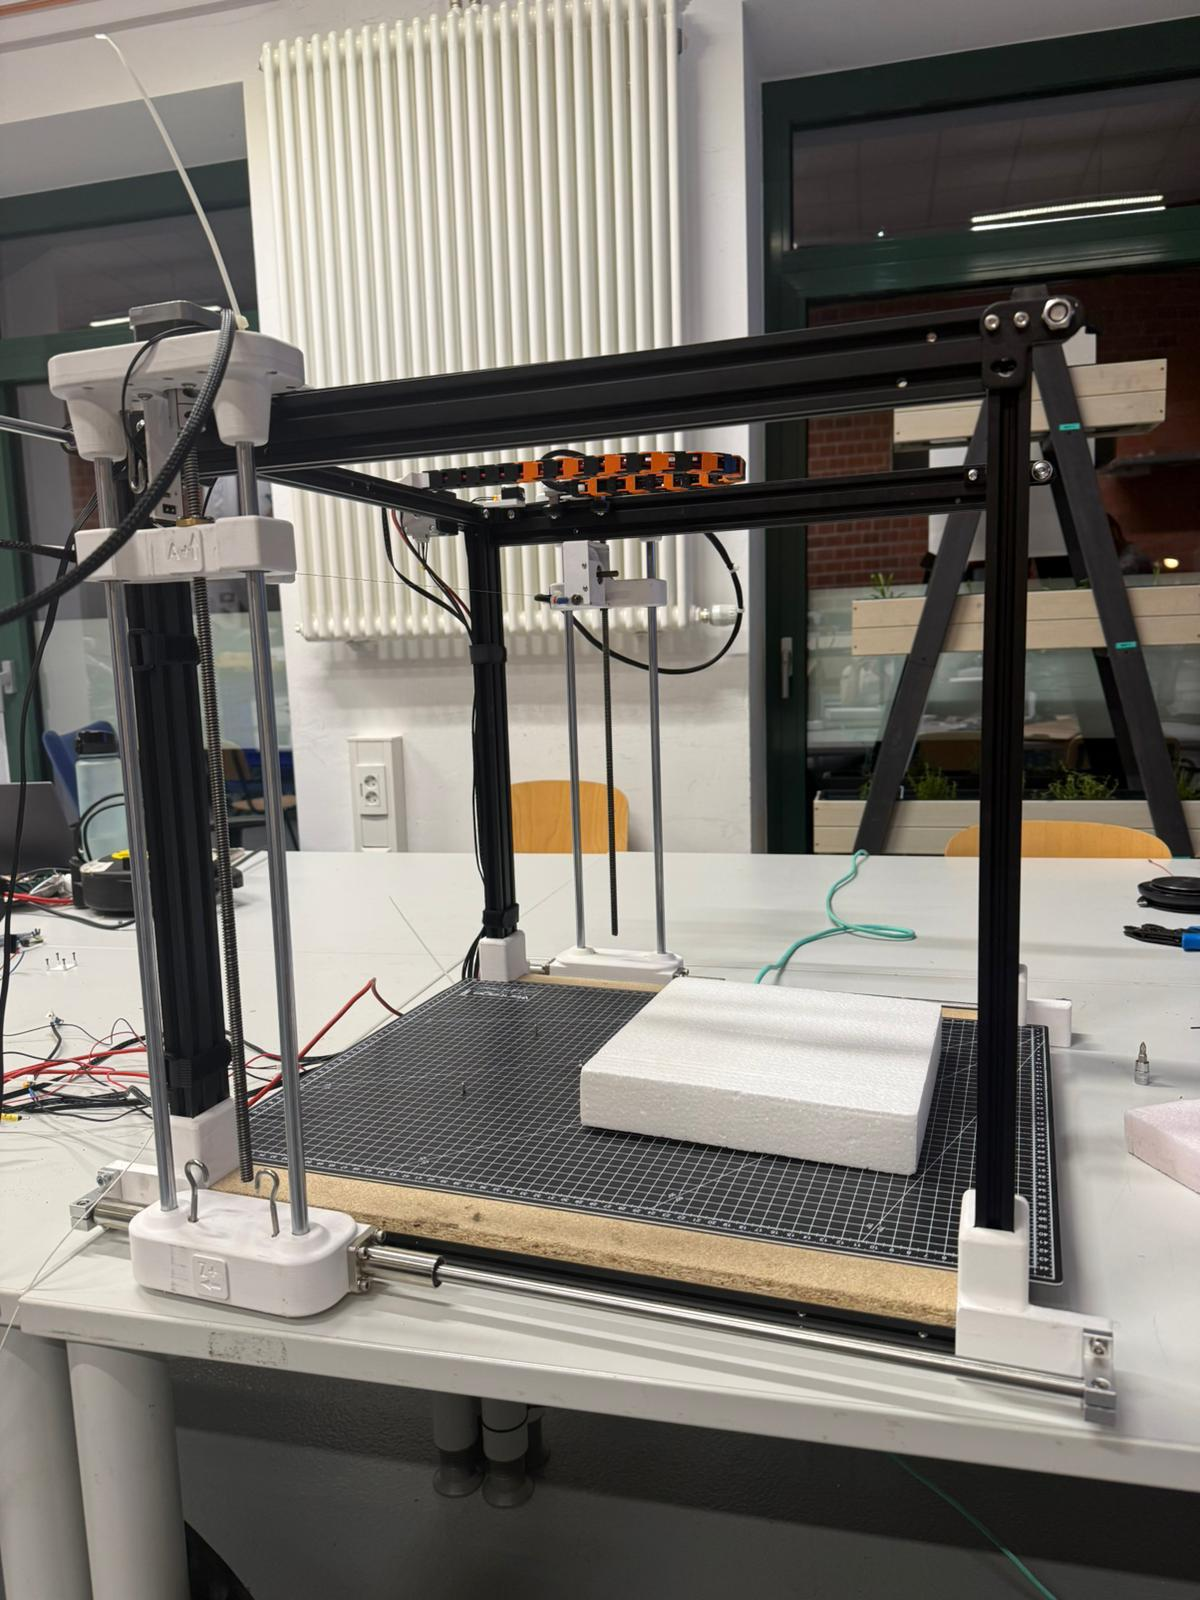
\includegraphics[height=4.7cm,width=\textwidth,keepaspectratio]{images/foto_aufbau_front}
      \\ \scriptsize Aufbau mit Styroporblock
    \end{column}
    \begin{column}{0.32\textwidth}
      \centering
      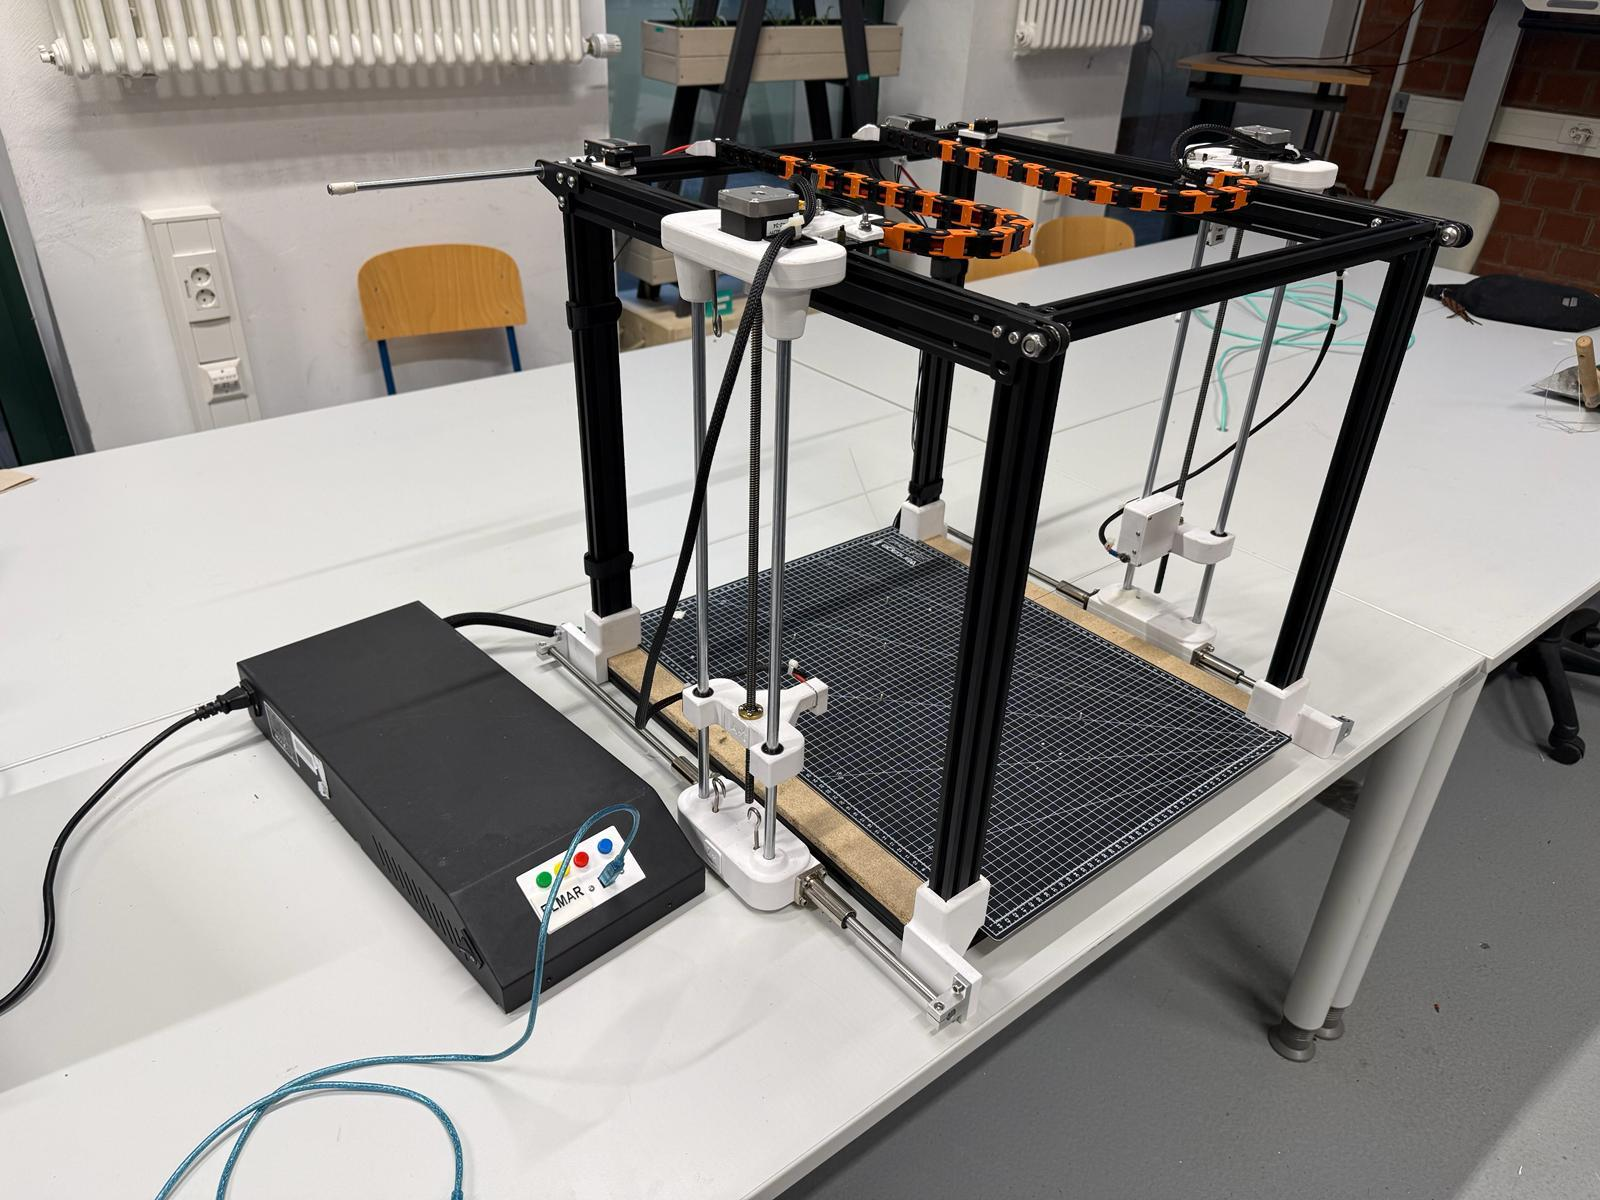
\includegraphics[height=4.7cm,width=\textwidth,keepaspectratio]{images/foto_aufbau_schraeg}
      \\ \scriptsize finaler Aufbau mit Steuerbox
    \end{column}
  \end{columns}
}

\STANDARD{Fotoeindrücke - Schnittversuche}
{
  \begin{columns}[T]
    \begin{column}{0.48\textwidth}
      \centering
      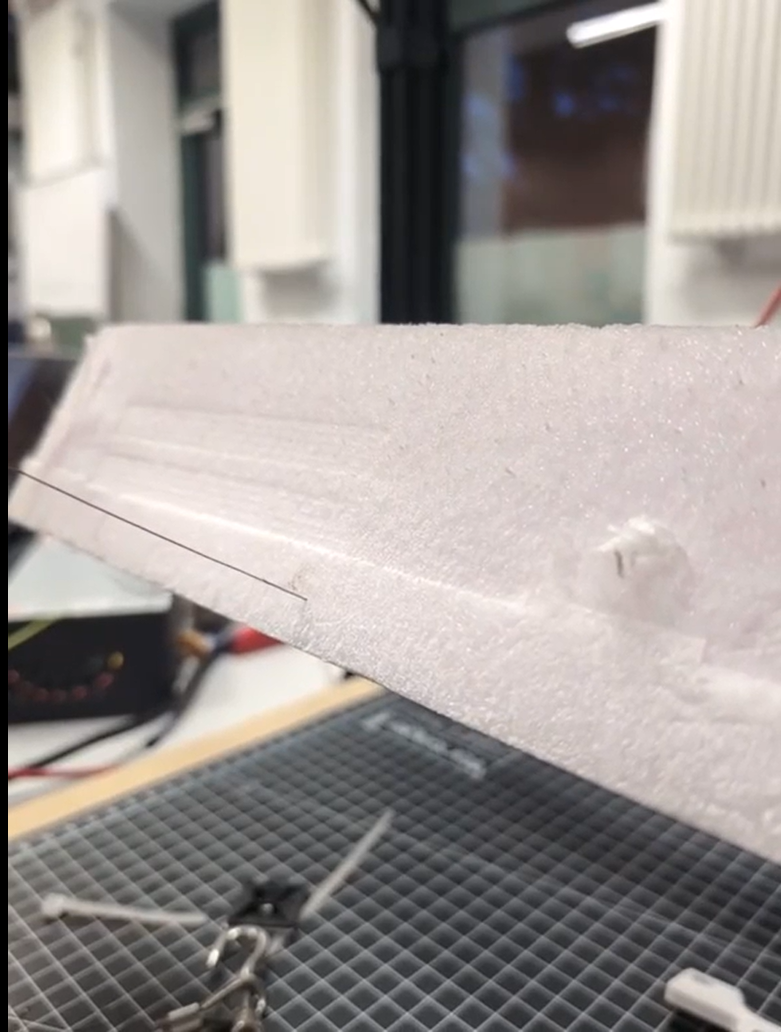
\includegraphics[height=5.1cm,width=0.98\textwidth,keepaspectratio]{images/foto_schnittkante}
      \\ \scriptsize Schnittkante im Styropor
    \end{column}
    \begin{column}{0.48\textwidth}
      \centering
      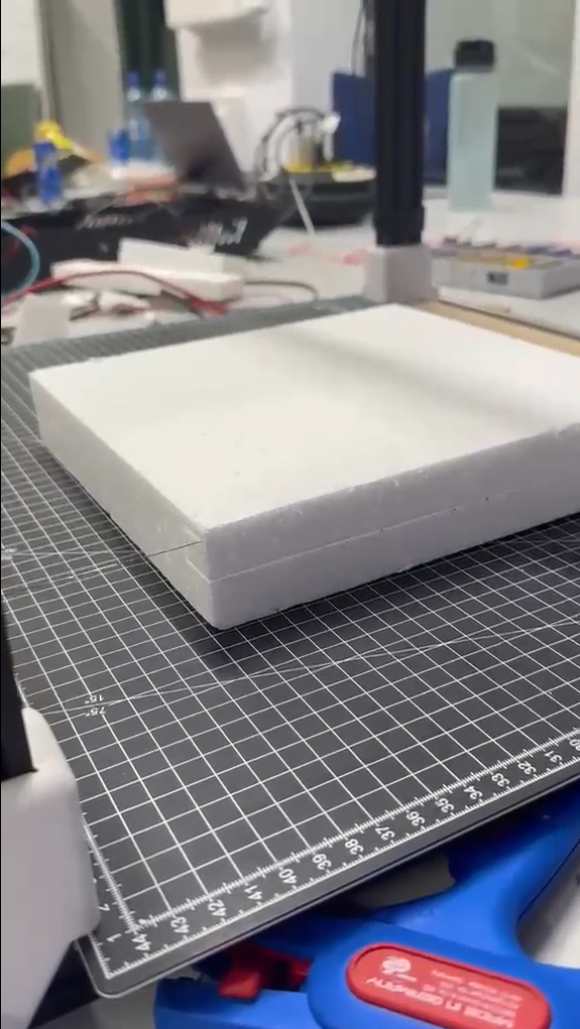
\includegraphics[height=5.1cm,width=0.98\textwidth,keepaspectratio]{images/foto_schaumblock}
      \\ \scriptsize Probeschnitt am Schaumstoffblock
    \end{column}
  \end{columns}
}

\Mysection{Fazit}

\STANDARD{Fazit}
{
  \begin{block}{Zusammenfassung}
    ELMAR zeigt, dass ein automatisierter Heiß Drahtschneider mit Arduino, GRBL, CNC-Shield und UGS grundsätzlich umsetzbar ist. Entscheidend für das Ergebnis ist nicht nur die Konstruktion, sondern vor allem die Abstimmung aus Mechanik, Elektronik, Software und Heizdrahtparameter.
  \end{block}

  \vspace{0.3cm}
  \begin{block}{Nächste sinnvolle Schritte}
    \begin{itemize}
      \item systematische Probeschnitte mit dokumentierten Temperatur- und Feedrate-Werten
      \item bessere Wiederholbarkeit der Drahtspannung
      \item Erweiterung um komfortablere lokale Bedienung oder Anzeige
    \end{itemize}
  \end{block}
}
